% This is samplepaper.tex, a sample chapter demonstrating the
% LLNCS macro package for Springer Computer Science proceedings;
% Version 2.20 of 2017/10/04
%
\documentclass[runningheads]{llncs}
%
\usepackage{graphicx}
% Used for displaying a sample figure. If possible, figure files should
% be included in EPS format.
%
% If you use the hyperref package, please uncomment the following line
% to display URLs in blue roman font according to Springer's eBook style:
% \renewcommand\UrlFont{\color{blue}\rmfamily}

\begin{document}
%
\title{Conversión de Mendoza a una ciudad sostenible}
%
%\titlerunning{Abbreviated paper title}
% If the paper title is too long for the running head, you can set
% an abbreviated paper title here
%
\author{Buccolini Á. \and Isgro I. \and
Martinez y Arenas L. \and Mellado M. \and
Neme O.}
%

% First names are abbreviated in the running head.
% If there are more than two authors, 'et al.' is used.
%
\institute{Facultad de Ingeniería, Universidad Nacional de Cuyo, Mendoza, Argentina }\\

%
\maketitle        % typeset the header of the contribution
%
\begin{abstract}
El siguiente artículo se enfocará en el análisis de factores a tener en cuenta para modernizar una ciudad de forma tal de reducir sus emisiones y lograr un funcionamiento más eficiente de la misma. Se hará un enfoque en la ciudad de Mendoza, donde se ubica la sede de la facultad.


\keywords{Cambio Climático \and Planificación Urbana  \and Energía Limpia \and Movilidad Sustentable  \and Eficiencia \and Sostenibilidad \and Ciudad de Mendoza}
\end{abstract}
%
\section{Introducción}
El cambio climático es uno de los mayores desafíos a los que se ha de enfrentar la humanidad. Prácticamente cada actividad que asegura el estilo de vida moderno emite gases de efecto invernadero (GEI), de no tomar medida alguna para reducir dichas emisiones, se agravará el impacto sobre la población a nivel mundial, incluyendo un aumento de la cantidad de desastres naturales y su magnitud, elevación de la temperatura media del planeta, entre otros problemas.\\

Para combatirlo se requiere un acuerdo entre todas las naciones, se deben tomar medidas que permitan llegar a reducir las emisiones y/o prácticamente eliminarlas. De allí surge el acuerdo de París en 2015, un hecho histórico que une a las naciones firmantes en una causa común para emprender acciones e inversiones necesarias para un futuro sostenible con bajas emisiones de carbono. En la actualidad, 197 países han adoptado el acuerdo, comprometiéndose a lograr una transición a economías de bajas emisiones de carbono.~\cite{ref_url8,ref_url10}\\

Sin embargo, los esfuerzos nacionales no serán suficientes sin cambios estructurales internos en cada uno de las ciudades más importantes del país, para luego trasladarlo a distritos de menor tamaño y emisiones. En la actualidad, más de la mitad de la población mundial vive en ciudades y se espera que dicha cantidad alcance un valor del 60\% para 2030. El rápido crecimiento urbano sin planificación implica infraestructuras y servicios inadecuados, ineficientes y sobrecargados, lo cual aumenta las emisiones.\\

En consecuencia, es necesario que cada ciudad invierta en medidas de sostenibilidad y de esta forma mejorar la calidad de vida de cada uno de sus habitantes y al mismo tiempo colaborar en el esfuerzo a nivel nacional y mundial para mitigar el cambio climático.


\section{Cambio climático y organizaciones}
\subsection{Influencia de las ciudades}
Uno de los Objetivos de Desarrollo Sostenible (ODS) de la Organización de las Naciones Unidas (ONU) establecidos para el 2030 es \textit{“Lograr que las ciudades sean más inclusivas, seguras, resilientes y sostenibles”}. Este objetivo analiza la importancia de las ciudades en el crecimiento económico, dado que representan aproximadamente el 60\% del PBI mundial, pero también recalca su aporte al cambio climático, representando un 70\% de las emisiones y más del 60\% del uso de los recursos (incluyendo el 80\% del consumo de energía) a pesar de ocupar solo el 3\% de la superficie terrestre.\\

De esta forma, su crecimiento en los próximos años va a provocar un agravamiento del cambio climático, volviendo cada vez más vulnerables a aquellas ciudades que todavía no estén preparadas a los desastres naturales y se deberá reforzar la resiliencia urbana para evitar pérdidas humanas, sociales y económicas.~\cite{ref_url9}
\begin{figure}
\centering
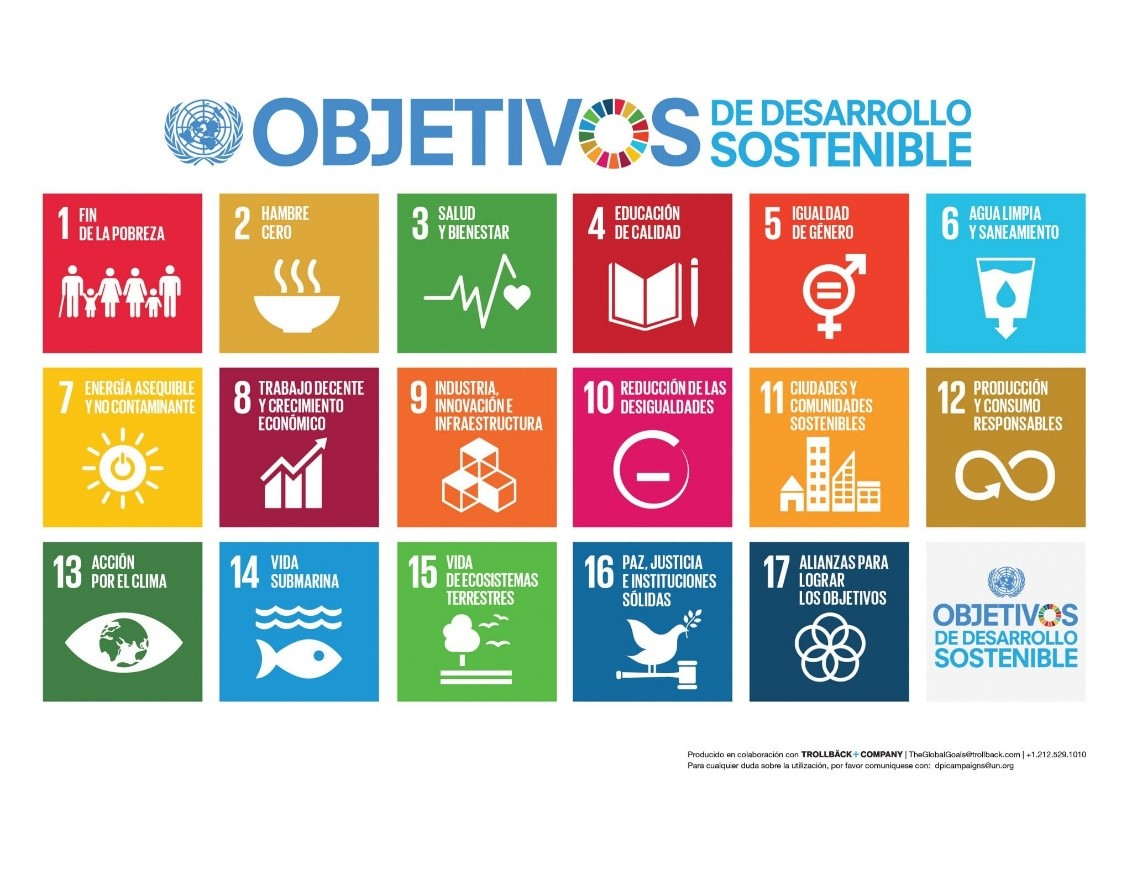
\includegraphics[width=10cm, height=7cm]{CEPAL.jpg}
\caption{Objetivos de Desarrollo Sostenible.} \label{fig1}
\end{figure}

En consecuencia, han surgido iniciativas para fomentar a las ciudades implementar políticas y acciones concretas para hacer frente al cambio climático y adaptarse a sus efectos debido a su aporte significativo a las emisiones y su vulnerabilidad a los impactos como olas de calor, sequías, etc. Una de estas iniciativas es el \textit{“Pacto Global de Alcaldes por el Clima y la Energía”}, el cual brinda apoyo a los firmantes en forma de asesoramiento técnico, intercambio de prácticas y acceso a financiamiento para proyectos relacionados con la energía y el clima.\\

Además involucra la identificación de riesgos climáticos actuales y futuros, las infraestructuras críticas y la toma de decisiones para que la sociedad se vuelva más resiliente ante los efectos adversos ya presentes.

\subsection{Pacto global de alcaldes }
El Pacto global de alcaldes es una de las alternativas de mayor interés para las ciudades dado que aborda tres cuestiones principales: 
\begin{itemize}
    \item \textit{Mitigación del cambio climático}. 
    \item \textit{Adaptación a los efectos adversos del cambio} 
    \item \textit{Acceso universal a energía segura, limpia y asequible}.~\cite{ref_url2}
\end{itemize}

Este brinda herramientas a las ciudades postulantes que permitan planificar su desarrollo y brinda acceso a créditos para llevar a cabo la transición a modelos sostenibles.


\section{Aspectos a considerar en la transición}
\subsection{Planificación urbana con bajas emisiones}

Esta propuesta hace referencia al diseño e implementación de políticas, programas, proyectos y/o acciones que promuevan la reducción del impacto del diseño urbano en las emisiones de GEI generados por las ciudades. Entre sus principios básicos se pueden identificar el ordenamiento territorial, diseño compacto y aprovechamiento del territorio, eficiencia energética en las construcciones, la gestión de residuos y la optimización y adecuación de sistemas de distribución, tratamiento y reutilización del agua.\\

Un aspecto importante es la densificación de las áreas existentes de forma inteligente y sostenible, alcanzando economías de escala en infraestructuras básicas (transporte, suministro y tratamiento de agua, electricidad), de forma tal de que pueda solventarse los costos de implementación de sistemas adicionales como equipos de bombeo, ascensores, etc. En general, los desarrollos de mayor densidad provocan costos de propiedad mayores, por lo que los ingresos públicos aumentarán en cuanto a impuestos a la propiedad.\\

Además, al aumentar la densidad poblacional se debe tomar medidas para lograr un desarrollo urbano sostenible. Por un lado, se debe implementar normas de construcción ecológica que permitan ahorrar energía y reducir las emisiones, fomentar la adquisición de electrodomésticos de consumo eficiente y estimular la creación de espacios verdes. Por otro lado, se debe tomar medidas para que la población concentrada en la ciudad pueda movilizarse de forma eficiente, por ejemplo, mediante la implementación de formas de transporte multimodal y aumentar la capacidad del transporte público. Esto incluye la creación de redes peatonales y ciclovías para conectar zonas de mayor de demanda de transporte e integrarlos a sistemas de movilidad sustentables como colectivos eléctricos, metro tranvías, etc.\\

A nivel mundial, las aglomeraciones más importantes permiten albergar una gran población y turistas debido a la integración de estos sistemas descriptos previamente. Además, se toman medidas que desalienten el uso del vehículo particular para limitar el tráfico circundante y la emisión de dióxido de carbono, como la dificultad para encontrar estacionamiento, limitación de tiempo de estacionamiento con parquímetros. Sin embargo, se debería continuar realizando igualmente una inversión en infraestructura vial para poder soportar el tráfico existente.~\cite{ref_book1}\\

En particular, la ciudad de Río de Janeiro, tras realizar un inventario de sus emisiones, ha decidido implementar un plan de acción que incluye agrandar la red de ciclovías, racionalizar los transportes colectivos e implementar corredores exclusivos para autobuses.~\cite{ref_url1}

\subsection{Energía limpia}
Los combustibles de origen fósil se han convertido en el suministro de energía predominante, a pesar de ser un recurso energético finito y la quema de los mismos resulta en grandes emisiones de dióxido de carbono. Para resolver este dilema, surge el concepto de energía limpia o renovable de forma tal de emancipar la producción de energía de la emisión de GEIs a la atmósfera. Existen muchas alternativas como paneles fotovoltaicos que permiten producir obtener energía eléctrica a partir de la radiación solar, energía hidroeléctrica que aprovecha la energía potencial del agua para luego convertirla en energía eléctrica, energía geotérmica, energía eólica, etc.\\

El sector público puede llevar a cabo políticas que fomenten la incorporación de tecnologías tanto en el sector público como en el privado. Otra políticas que se puede implementar es establecer objetivos de energía renovable en industrias, edificios y transporte, de forma tal de alentar acciones que favorezcan la transición a modelos limpios.~\cite{ref_url6}\\

El municipio vecino a la ciudad de Mendoza, Godoy Cruz, ha llevado a cabo políticas y acciones con el objetivo de lograr la neutralidad para 2030, al momento de realizar su inventario de emisiones, el consumo de energía representaba un 57\% de sus emisiones donde el 63\% incluye solamente el consumo residencial. En consecuencia, la municipalidad decidió tomar medidas para fomentar el uso de energías limpias e interiorizar a la población de sus beneficios mediante su difusión.\\

Mediante la implementación de tecnologías de aprovechamiento de energía solar, se ha resuelto problemas propios de los ciudadanos como seguridad y, al mismo tiempo, se genera energía cuyo sobrante retorna a la red. Entre estas políticas se tiene:\\

\begin{itemize}
    \item \textit{Solmáforos}: incorporan un sensor UV donde el color del dispositivo indica el nivel de exposición a radiación solar. Además, permiten la carga de dispositivos e incluyen un mecanismo de seguridad mediante un botón que llama al 911. 
    \item \textit{Implementación de paneles solares en edificios públicos}: se utiliza paneles fotovoltaicos para la iluminación del edificio, se utiliza también la energía solar para la producción de agua caliente y la instalación de artefactos de luminaria LED de bajo consumo.
    \item \textit{Incentivos crediticios a comercios y residentes para instalación de paneles solares}.~\cite{ref_url4,ref_url5}
\end{itemize}

\subsection{Transporte y movilidad sostenible}
La planificación tradicional de las ciudades ha considerado el transporte necesario para el desarrollo económico. Esto ha provocado que se desarrollen infraestructuras de transportes para poder acomodar el crecimiento de la demanda de vehículos privados. Sin embargo, este modelo de transporte urbano presenta varios problemas como la contaminación del aire, el consumo excesivo de energía y el aumento de la congestión de las vías de tránsito.\\

Por ello surge la movilidad sustentable que busca lograr el movimiento eficiente, limpio, y seguro de personas y bienes en las ciudades. Para ello se propone utilizar vehículos cuyo consumo energético sea más eficiente mediante el uso de materiales ligeros y/o el aumento de la ocupación a partir del despliegue de medios de transporte sustentables. Además, se busca minimizar el número de vehículos particulares y sus emisiones, sustituyendo combustibles fósiles por biocombustibles, electricidad o hidrógeno. Para que el uso de estos dos últimos sea eficiente, se deben producir mediante fuentes con bajas emisiones de GEIs como las detalladas previamente.\\

Para combatir el aumento de la congestión, los problemas ambientales y la reducción de la calidad del transporte público, se debe desarrollar un plan integral de movilidad sustentable que comprenda:\\

\begin{itemize}
    \item \textit{Servicio público urbano completo}: se debe diseñar el sistema de transporte público de forma integrado, incentivando su uso a partir de servicios de calidad, formas de acceder a información completa, desarrollo de vías exclusivas de autobuses, metro tranvía. Esto último se puede integrar con estaciones de alquiler de bicicletas u otros medios similares que puedan hacer uso de las redes ciclovías.\\
    \item \textit{Control de tránsito}: cada ciudad debe establecer estrategias para limitar el uso de los vehículos particulares para aquellos que realmente lo requieran. Por ejemplo, se puede establecer límites de estacionamiento.\\
    
\end{itemize}

En la ciudad de Rosario, se estableció un sistema de movilidad sustentable que consiste en la creación de vías exclusivas para autobuses, la adquisición de autobuses eléctricos los cuales tienen una mayor vida útil y son más limpios. Además, se establecieron 52 estaciones de bicicletas para recorrer las ciclo vías exclusivas establecidas en la ciudad. Por último, se tomaron medidas para desincentivar el uso de coches privados mediante restricciones de aparcamiento.~\cite{ref_url3}\\



\section{Análisis Ciudad de Mendoza}
La Ciudad de Mendoza es un oasis con gran concentración de población ubicado en el norte de la provincia, es alimentada por la cuenca del Río Mendoza (y también por aguas subterráneas), a su vez este es alimentado por las nevadas y deshielo de glaciares. Uno de los impactos más importantes del cambio climático es el aumento de la temperatura.  A partir de datos del Servicio Meteorológico Nacional (SMN), se ha tenido un incremento de la temperatura media anual en unos 0,6°C en el periodo 1950-2010, esto implica un aumento del caudal de invierno/primavera a expensas del correspondiente al fin del verano, dado que se produce antes el derretimiento de la nieve y una aceleración del deshielo de los glaciares en cordillera.~\cite{ref_url11}\\

Otro impacto observado es el agravamiento de las lluvias y tormentas de granizo ( a pesar de que se estima que las precipitaciones se reduzcan de 340 a 304mm anuales en el período 2015-2040), esto implica inundaciones, caídas de ramas y árboles, corte de servicios y daños a infraestructuras. \\

Finalmente, el crecimiento de la población requiere de una planificación inteligente de la expansión de la ciudad.\\

En 2020, la ciudad estableció una política llamada \textit{Plan Local de Acción Climática}, que consiste en una herramienta de planificación estratégica para gestionar recursos técnicos y económicos para trascender hacia una ciudad eficiente y, por sobre todo, resiliente. Según el Acuerdo de París, para limitar el aumento de la temperatura global a 1,5°C, las emisiones de gases de efecto invernadero (convertidos a equivalentes de dióxido de carbono) se deberían recortar a un 51\%. Se tienen los siguientes valores de emisiones de gases de efecto invernadero:~\cite{ref_url13}

\begin{table}
\centering
\caption{Análisis de emisiones de gases de efecto invernadero de la Ciudad de Mendoza.}\label{tab1}
\begin{tabular}{|l|l|l|}

\hline
Año  &  Variación porcentual & Emisión resultante (TCO_2e)\\
\hline
2018 & -  & 861.985\\
2019 &  -12\% & 756.865\\
2020 & -17\% & 628.444\\

\hline
\end{tabular}
\end{table}

Según datos del INDEC, la población de la Ciudad de Mendoza crecerá en un 23\% en el periodo 2020-2030, por lo que se deben tomar medidas para compensar el consecuente aumento de las emisiones de GEIs.~\cite{ref_url12}\\

Desde el punto de vista de la movilidad, la Ciudad ya ha establecido medidas como créditos para compras de bicicletas para particulares, adquisición de autobuses eléctricos y una normativa que requiere que las playas de estacionamiento tengan espacio para bicicletas y ampliación de la red de ciclo vías.A pesar de todo esto, el 46\% de las emisiones del año 2020 correspondieron al transporte.~\cite{ref_url13}\\


Para lograr un impacto mayor en las emisiones se deben establecer medidas más intensas como:

\begin{itemize}
    \item \textit{Reemplazo total de la flota de autobuses a combustible fósil por eléctricos}: esto volverá más atractivo el transporte público debido a mayores comodidades y reducirá las emisiones.
    
    \item \textit{Estímulos a empresas}: el sector público puede brindar beneficios para fomentar dentro del sector privado el uso de vehículos eléctricos, bicicletas, scooters o car pooling, entre otros.

    \item \textit{Incentivo a uso de vehículos eléctricos}: El municipio puede brindar beneficios a aquellos que adquieran un vehículo de este tipo. Se debe incorporar puestos de carga para hacer más atractivo la compra de estos.

    \item \textit{Incentivo a traslado peatonal o por bicicleta}: para ello se debe llevar a cabo un mantenimiento de las veredas, expansión de bici sendas e incluso implementar nuevas calles peatonales.

    \item \textit{Desalentar el uso de coche privado}: se puede establecer zonas de exclusión de estacionamiento, fomentar el uso compartido de vehículos, etc. Esto no sólo reducirá las emisiones, sino que también permitirá descongestionar las vías de tránsito, principalmente las de acceso a la ciudad en los horarios pico.

    \item \textit{Movilidad multimodal}: establecimiento de estaciones de alquiler de bicicleta en puntos de importancia de la ciudad en conjunto con paradas de autobuses, beneficios en el "trasbordo" de un medio a otro.
\end{itemize}

Por otro lado, se debe llevar a cabo una planificación urbana eficiente que sea capaz de albergar esta población creciente. La capital mendocina sufre de un fenómeno llamado islas de calor, focos donde se concentra el calor, por lo que se tienen mayores temperaturas en sectores particulares de la ciudad. Para esto, se deben implementar normas constructivas que utilicen materiales que absorban menos calor y fomentar las áreas verdes en las construcciones nuevas.\\

En particular, la Ciudad de Mendoza cuenta con un sector poco explotado que es el piedemonte. Este no ha sido completamente poblado debido a razones de movilidad como la lejanía del centro de la ciudad, baja conveniencia en el uso del transporte público; escasez de ciclovías y distancias muy grandes para ser recorridas peatonalmente. Se puede implementar algunas de las medidas de movilidad ya descriptas previamente para volver más atractivo este sector de la ciudad.\\

Además, se debe implementar un código de construcción que establezca las secciones donde se deba aplicar medidas extras de seguridad para hacerle frente a los deslizamientos de suelos y las posibles consecuencias del mismo, dado que el piedemonte mendocino es una zona propensa a aluviones.\\

En cuanto al sector energético, se tiene que representa el 43\% de las emisiones de la ciudad, por lo que se debe considerar medidas que permitan la generación de energía desde fuentes limpias. Una de las características de la ciudad de Mendoza es que tiene una gran cantidad de días de sol al año, por lo que tiene un enorme potencial en la generación de energía solar.~\cite{ref_url13}\\

Actualmente, se tienen paneles solares instalados en la Nave Cultural y el Gimnasio Municipal N°2 con una potencia de 140 kW. Esto resulta un buen paso inicial y se debería implementar más políticas como:

\begin{itemize}
    \item \textit{Incorporación de paneles solares para edificios municipales}: permitirá cubrir parte de su consumo y se puede instalar calefones que aprovechen la energía solar para calentar el agua de los empleados.
    
    \item \textit{Créditos a comercios y residentes para la adquisición de paneles solares}: se generaría una nueva dinámica donde se incluye el "prosumidor", parte de la energía generada va a ser vendida a la red y otra parte va a ser consumida.

    \item \textit{Torres solares}: Se pueden instalar en espacios públicos, por lo que pueden funcionar como puestos de carga de cualquier dispositivo eléctrico y también como calentador de agua para mate.

    \item \textit{Implementación de equipos para eficiencia energética en edificios municipales}: se puede instalar sensores de presencia que detecten si es necesario iluminar un área y se puede programar el apagado automático de equipos.

    \item \textit{Recambio de luminaria}: se debe instalar luces de bajo consumo para derrochar lo mínimo posible de forma tal de aprovechar la energía limpia producida con las medidas anteriores.

    \item \textit{Instalación de medidores inteligentes}: para controlar de forma correcta el aporte de los "prosumidores" y tomar medidas con aquellos particulares que cometan fraude eléctrico. 
\end{itemize}

\section{Conclusiones}

El cambio climático es un hecho que va a impactar fuertemente en nuestra sociedad en los años venideros, las ciudades se encuentran en posición de tomar medidas que ayuden a mitigarlo y adaptarse a sus efectos sin necesidad de lograr un gran consenso o esperar planes nacionales.\\

En particular, para ciudades ubicadas en países de menor desarrollo económico es fundamental tomar acción dado que cuentan con mayores sectores de población vulnerables al cambio climático. Iniciativas como el Pacto Global de Alcaldes son esenciales para orientarlas en el proceso de transición y poder acceder a créditos, que de no tenerlos, harían imposible llevar a cabo cualquier empréstito de esta magnitud.\\

La pandemia de COVID-19 demostró la vulnerabilidad ante una perturbación a nivel mundial por falta de preparación. Sin embargo, se aprendió que la población puede trabajar en conjunto en pos de un objetivo en común y esto resulta un gran punto de partida para repensar el desarrollo de nuestras ciudades desde una perspectiva sostenible y resiliente.


\begin{thebibliography}{8}

\bibitem{ref_url8}
Organización de las Naciones Unidas. The Paris Agreement. ~\url{https://www.un.org/en/climatechange/paris-agreement}

\bibitem{ref_url10}
Naciones Unidas para el cambio climático . Acuerdo de París. ~\url{https://unfccc.int/es/most-requested/que-es-el-acuerdo-de-paris}

\bibitem{ref_url9}
Organización de las Naciones Unidas. Sustainable Development Action - Sustainable cities and communities. ~\url{https://www.un.org/sustainabledevelopment/cities/}

\bibitem{ref_url2}
Global Covenant of Mayors for Climate and Energy. Sobre el pacto. ~\url{https://pactodealcaldes-la.org/sobre-el-pacto/}

\bibitem{ref_book1}
Jenks, M., Burgess, R.: Compact Cities: Sustainable Urban Forms for Developing Countries. 1ra edn. Spon Press, EEUU y Canadá (2004)


\bibitem{ref_url1}
Programa Internacional de Cooperación Urbana (IUC,2019). El futuro de nuestras ciudades.~\url{https://iuc-la.eu/wp-content/uploads/2020/05/FuturoNuestrasCiudades\_170919\_baja.pdf}.


\bibitem{ref_url6}
Programa Internacional de Cooperación Urbana. Sector 2 - Energía Limpia.~\url{https://iuc-la.eu/wp-content/uploads/2020/03/ES\_EL\_1\_Sector\_2\_-\_Energi\%cc\%81a\_Limpia.pdf}


\bibitem{ref_url4}
Global Covenant of Mayors for Climate and Energy (2022). Ejemplo de accesibilidad energética rumbo a la neutralidad de carbono.~\url{https://pactodealcaldes-la.org/wp-content/uploads/2022/05/GCoM-estudio-de-caso-Godoy-Cruz-1.pdf}

\bibitem{ref_url5}
Mastrángelo y Mora (2020). Godoy Cruz: Caso Solmáforo - Autos y Bicis eléctricas.~\url{https://iuc-la.eu/wp-content/uploads/2020/03/Godoy\_Cruz\_-\_Solmaforo\_Torre\_para\_calentar\_agua\_y\_telefonos\_celulares\_Auto\_y\_bicis\_electricas.pdf}

\bibitem{ref_url3}
Programa Internacional de Cooperación Urbana. Estudios de caso. ~\url{https://iuc-la.eu/estudios-de-caso/}

\bibitem{ref_url11}
Servicio Meteorológico Nacional (SMN). Monitoreo climático ~\url{https://www.smn.gob.ar/clima/vigilancia}

\bibitem{ref_url13}
Municipalidad de Mendoza. Plan Local de Acción Climática. 

\bibitem{ref_url12}
Instituto Nacional de Estadísticas y Censos (INDEC). Censos ~\url{https://www.indec.gob.ar/indec/web/Nivel3-Tema-2-41}


\end{thebibliography}
\end{document}

